\chapter{The Weyl Pseudometric}\label{chapter:Weyl}

In this chapter we introduce the Weyl pseudometric that is one of the crucial tools in our proof of a generalized Krieger's Theorem (Theorem \ref{Krieger2}).
%
Given a dynamical system $(X,G)$, the Weyl pseudometric $D_W$ is defined on $X^G$ and thus via a natural identification of points $x\in X$ with their trajcetories $\und{x}_G\in X^G$ induces a pseudometric structure on $X$.
%
A good example is when $X=\{0,1\}^G$ with the shift action, in which case $D_W$ is equivalent (see Theorem~\ref{thm:shift_equiv_weyl}) to a metric on $X$ where the distance between $x,y\in \{0,1\}^G$ is the {\it upper Banach density} of the set of indices at which $x$ and $y$ differ, i.e., $D_W(x,y)=D^\star \inparen{\{g\in G: x(g)\neq y(g)\}}$.
%
Given that example, one might already expect that it interacts quite well with entropy, which indeed is the case, as demonstrated in Section~\ref{section:entropy_q-u_cont}.


Along with the Weyl pseudometric, in this chapter, we also study the related notion of Banach density as well as the Besicovitch pseudometric that, in a certain sense can be seen as a ``simpler'' variant of Weyl.
%
Using these two notions we state and prove alternative formulas for the Weyl pseudometric (see Theorem \ref{uniEquivDw}, Lemma \ref{lem:Dw_is_supDB} and Lemma \ref{lem:2formulasDw}) that are generally useful in this thesis, but might also be of independent interest.

\section{Densities in Amenable Groups}\label{section:density}
Before we proceed with the definition of the Weyl pseudometric let us start with a section that introduces the notion of Banach density in amenable groups.
%
This is an adaptation of the familiar number-theoretic notion of density of a subset of $\N$ adjusted to our setting.
%
This notion of density is then useful to define a handy, equivalent formula for the Weyl pseudometric that we actually work with.
%
As a conclusion of this section we show a simple (yet surprisingly tricky to prove) formula for the Banach density of a special family of sets in $G$ that can be thought of as ``periodic''.

We start by introducing the basic notation. Recall that by $\Fin(G)$ we denote the collection of all finite non-empty subsets of $G$ and by $\cP(A)$ we mean the power set of a set~$A$, i.e., the collection of all its subsets. We use $\F$ to denote a \Folner sequence $\F = \{F_n\}_{n\in \N}$ in $G$. 
%
Whenever a $\sup_{\F}$ appears in a formula, it is meant to be the supremum over all \Folner seqences in $G$. 
%
\begin{defn}[Asymptotic densities and Banach densities]
The following formulas define the upper and lower asymptotic density of  $A\subseteq G$  with respect to a \Folner sequence $\F=\{F_n\}_{n\in\N}$:
\begin{enumerate}
\item {\bf (Upper asyptotic density)} \hspace{5mm} $\displaystyle\dbar_{\F}(A)\defeq \limsup_{n\to\infty}\frac{|A\cap F_n|}{|F_n|},$
\item {\bf (Lower asyptotic density)} \hspace{5.7mm}  $\displaystyle \underline d_{\F}(A)\defeq \liminf_{n\to\infty}\frac{|A\cap F_n|}{|F_n|}. $
\end{enumerate}
If $\dbar_{\F}(A)=\underline d_{\F}(A)$, then we say that $A$ has the \emph{natural density} with respect to $\F$ and we write $ d_{\F}(A)=\dbar_{\F}(A)$.

The upper and lower Banach densities of $A\subseteq G$ are given by
\begin{enumerate}
\item {\bf (Upper Banach density)} \hspace{5mm} $\displaystyle D^\star(A)\defeq \inf_{F\in\Fin(G)}\sup_{g\in G}\frac{|A\cap Fg|}{|F|},$
\item {\bf (Lower Banach density)} \hspace{5.7mm}  $\displaystyle D_\star(A)\defeq 1-D^\star(G\setminus A). $
\end{enumerate}
If $D_\star(A)=D^\star(A)$, then we say that $A$ has the \emph{Banach density} $D(A)=D^\star(A)$.
\end{defn}

\noindent
Notice that the above definition of Banach density does not require the group $G$ to be amenable.
%
Unfortunately this particular definition is not convenient to work with densities, thus we state the following alternative formulations that were first obtained in~\cite{DHZ16} and~\cite{BBF10}.

\begin{lem}
For $A\subseteq G$, the upper Banach density is given by:
\begin{enumerate}
\item \cite[Lemma 2.9]{DHZ16}\hspace{5mm} $\displaystyle D^\star(A)=\lim_{n\to\infty}\sup_{g\in G}\frac{|A\cap F_ng|}{|F_n|},$ \\ where $\F=\{F_n\}_{n\in\N}$ is an arbitrary \Folner sequence. In particular, the above limit exists and does not depend on the choice of $\mathcal F$;
\item \cite[Lemma 3.3]{BBF10} \hspace{5mm}  $\displaystyle D^\star(A) =  \sup_{\F} \dbar_{\F}(A).$ \\
(Recall that $\sup_{\F}$ means that the supremum is taken over all \Folner sequences in $G$.)
\end{enumerate}
\end{lem}
\noindent
In the following, we may use these formulas without further reference.


We now derive a rather simple and intuitive formula (in~Lemma~\ref{ECdensity}) for the upper Banach density of ``periodic'' sets.
%
Such sets are crucial in the proof of Theorem~\ref{Krieger2}.
%
We first prove some preliminary results.

Observe the following relation between upper and lower asymptotic densities:

\begin{lem}\label{lem:upper-lower}
If $\F$ is a \Folner sequence and $A\subseteq G$, then 
$
\dbar_{\F}(A)=1-\und{d}_{\F}(G\setminus A).
$
\end{lem}

\begin{proof}
Fix a \Folner sequence $\F=\{F_n\}_{n\in\N}$ and let $A\subseteq G$. Then
\begin{align*}
\und{d}_{\F}(G\setminus A)&=\liminf_{n\to\infty}\frac{|(G\setminus A)\cap F_n|}{|F_n|} \\
&=\liminf_{n\to\infty}\frac{|F_n\setminus (A\cap F_n)|}{|F_n|} \\
&= \liminf_{n\to\infty}\inparen{1- \frac{|A\cap F_n|}{|F_n|} } \\
& = 1- \limsup_{n\to\infty} \frac{|A\cap F_n|}{|F_n|} \\
&=1-\dbar_{\F}(A). \qedhere
\end{align*}
\end{proof}

\noindent
Next we prove a simple lemma that is a straightforward consequence of amenability.
\begin{lem}\label{lem:Folner_inv}
If $\F=\inbrace{F_n}_{n\in\N}$ is a \Folner sequence in $G$ and $F\in\Fin(G)$, then for any $\eps>0$ and for all $n$ large enough, one has $|FF_n\Delta F_n|<\eps|F_n|$.
\end{lem}

\begin{proof}
Fix $\eps>0$. Since $\F$ is F{\o}lner, for every $f\in F$ there exists $N_f\in\N$ such that for every $n\geq N_f$ one has
\[
\frac{|fF_n\Delta F_n|}{|F_n|}<\frac{\eps}{|F|}.
\]
Define $N\defeq \max\{N_f: f\in F\}$. Then for every $n\geq N$ we have
\[
\frac{1}{|F_n|}\inmodul{\inparen{\bigcup_{f\in F}fF_n}\Delta F_n}\leq \frac{1}{|F_n|}\inmodul{\bigcup_{f\in F}\inparen{fF_n\Delta F_n}}\leq\sum_{f\in F}\frac{\inmodul{fF_n\Delta F_n}}{|F_n|}<\eps. \qedhere
\]
\end{proof}



\begin{figure}\label{fig:F-hull}
\centering
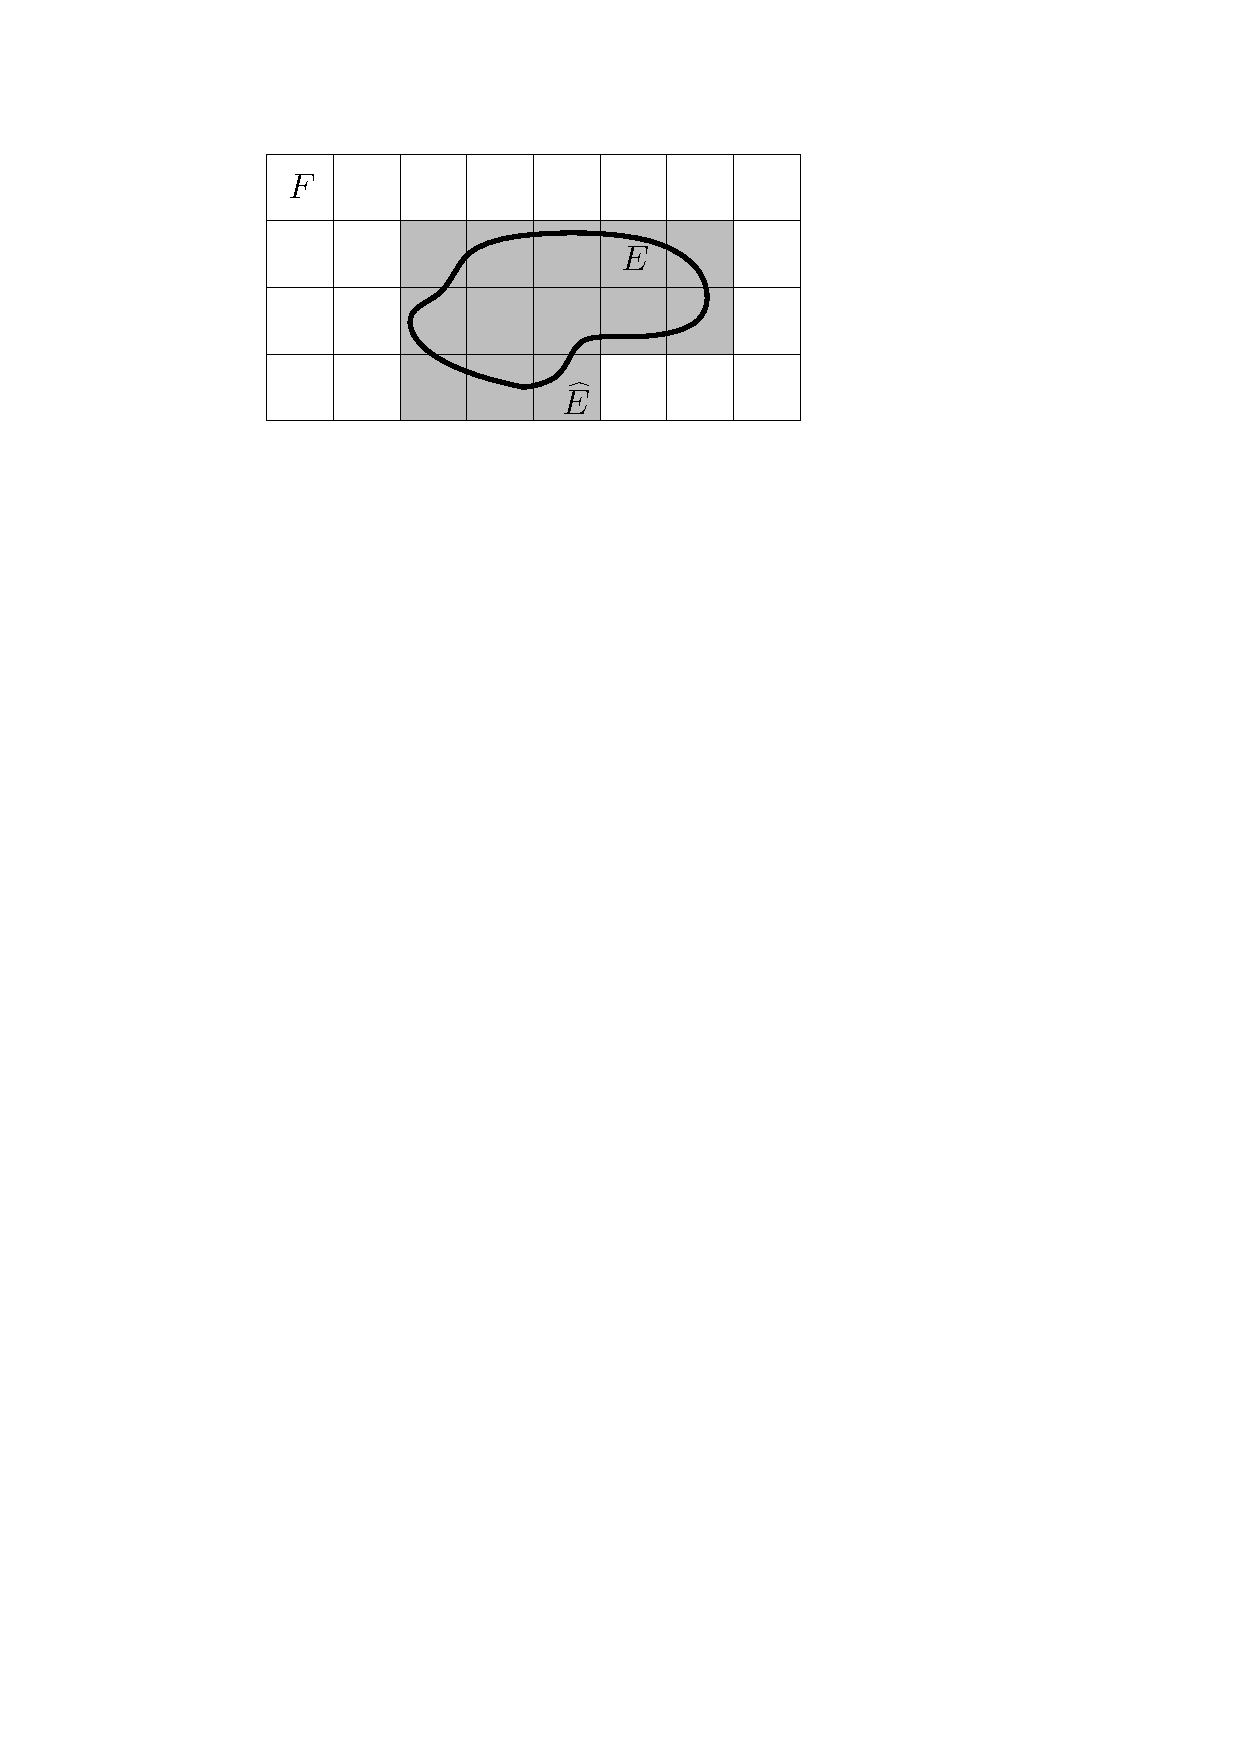
\includegraphics[scale=1]{Graphics/E_hat_densities.pdf}
\caption{An illustration for Lemma \ref{lem:hatE-E}. We can see a set $E\in\Fin(G)$ (the interior of the area marked with the fat line) and the set $\widehat E$ defined in Lemma \ref{lem:hatE-E}  (the grey area). The set $\widehat E$ is the sum of shifted copies of $F$ that intersect $E$ (a copy of $F$ is depicted as a single square). }
\end{figure}
\noindent 
The following technical lemma is the final preparation necessary to derive Lemma~\ref{ECdensity}.
\begin{lem}\label{lem:hatE-E}
Let $F\subseteq G$ be a monotile (see Definition \ref{def:tile}), $C\subseteq G$ be a set of centers for $F$, and let  $\eps>0$. If a set $E\in\Fin(G)$ satisfies $|FF^{-1}E\Delta E|<\eps|E|$, then for 
\[
\widehat E\defeq\bigcup\{Fc:c\in C \text{ is such that } Fc\cap E\neq\emptyset\}.
\]
the following inequality holds
\begin{equation*}\label{eq:1}
|\widehat E|-|E|\leq\eps |E|.
\end{equation*}
\end{lem}
\begin{proof}
Notice that $E\subseteq FF^{-1}E$ since $e\in F$. This implies 
\begin{equation*}\label{eq:2}
|FF^{-1}E\Delta E| = |FF^{-1}E\setminus E|= |FF^{-1}E|-|E|.
\end{equation*}
Hence it is enough to prove that
$
|\widehat E|\leq |FF^{-1}E|
$
since $|FF^{-1}E\Delta E|<\eps|E|$.
We show that $\widehat E\subseteq FF^{-1}E$.
Choose $g\in\widehat E$. Then there exists exactly one $c_g\in C$ and exactly one $f_g\in F$ such that $g=f_gc_g$. 
By the definition of $\widehat E$, there exists $h\in E$ such that $h\in Fc_g$. 
That means that $h=f_hc_g$ for some $f_h\in F$. 
Combining these two observations, we obtain $g=f_gf_h^{-1}h\in FF^{-1}E$.
\end{proof}

\noindent
Finally, we are ready to prove the main technical result of this section.
\begin{lem}\label{ECdensity}
If 
%$\F=\{F_n\}_{n\in\N}$ is a \Folner sequence, 
$F\subseteq G$ is a monotile with the associated set of centers $C$ and $E\subseteq F$, then 
\[
 D^\star(EC)=\frac{|E|}{|F|}.
 \]
\end{lem}

\begin{proof} 
Let $\F=\{F_n\}_{n\in\N}$ be a \Folner sequence in $G$ and let $\eps>0$. For each $n\in\N$ we define (see Figure \ref{fig:F-hull})
\[
\widehat F_n\defeq\bigcup\{Fc:c\in C \text{ satisfies } Fc\cap F_n\neq\emptyset\}.
\]
By Lemma \ref{lem:Folner_inv}, there exists $N\in\N$ such that $|FF^{-1}F_n\Delta F_n|<\eps|F_n|$ for every $n\geq N$. Then for any $n\geq N$ one has
\begin{align}
\frac{|EC\cap F_n|}{|F_n|}
&=\frac{|EC\cap(\widehat F_n\setminus(\widehat F_n\setminus F_n))|}{\inmodul{F_n}} \quad\mbox{(since  $F_n\subseteq \widehat F_n$)} \nonumber\\
&= \frac{|EC\cap\widehat F_n|}{|F_n|}-\frac{|EC\cap (\widehat F_n \setminus F_n)|}{|F_n|} \nonumber\\ 
&\geq\frac{|EC\cap \widehat F_n|}{|F_n|} - \frac{|\widehat F_n|-|F_n|}{|F_n|} \nonumber\\
&\geq \frac{|EC\cap \widehat F_n|}{|F_n|} - \frac{\eps|F_n|}{|F_n|} \quad\text{(by Lemma \ref{lem:hatE-E})} \label{eq:EC}\\
&\geq \frac{|EC\cap \widehat F_n|}{|\widehat F_n|} - \eps \nonumber\\
&=\frac{|E||\{c\in C: Fc\cap F_n\neq\emptyset\}|}{|F||\{c\in C: Fc\cap F_n\neq\emptyset\}}-\eps \nonumber\\
&= \frac{|E|}{|F|}-\eps. \nonumber
\end{align}
Since $\eps$ was arbitrary and the above inequality holds for all sufficiently large $n$, we obtain 
\[
\dbar_{\F}(EC)\geq \und{d}_{\F}(EC)\geq \frac{|E|}{|F|}.
\] 
Replacing $E$ by $E':=F\setminus E$, we obtain
\[
\und{d}_{\F}(E'C)\geq \frac{|E'|}{|F|}.
\]  
Since $G\setminus E'C = EC$, using the relation between upper and lower asymptotic density (see Lemma~\ref{lem:upper-lower}), we obtain
\[
\dbar_{\F}(EC)=1-\und{d}_{\F}(E'C)\leq 1 - \frac{|E'|}{|F|} = \frac{|E|}{|F|}. 
\]
Hence 
\[
\dbar_{\F}(EC)=\frac{|E|}{|F|}.
\]
Since $\F$ was arbitrary, taking the supremum over all \Folner sequences, one has
\[
D^\star(EC)= \frac{|E|}{|F|}. \qedhere
\]
\end{proof}
\noindent 
As a corollary from the above lemma we obtain the following 
\begin{lem}\label{lem:Dstar_properties}
Let $F\subseteq G$ be a monotile with associated set of centers $C\subseteq G$.
If $A\subseteq G$ and $B\subseteq G$ are such that $A=E_1C$ and $B=E_2C$ for some $E_1,E_2\subseteq F$, then
\begin{enumerate}
\item $A\subseteq B$ implies $D^\star(A\setminus B)= D^\star(A)-D^\star(B)$,
\item  $A\cap B=\emptyset$ implies $D^\star(A\cup B)= D^\star(A)+D^\star(B)$.
\end{enumerate}
\end{lem}

\begin{proof}
Clearly $A\subseteq B$ is equivalent to $E_1\subseteq E_2$, and $A\cap B=\emptyset$ is equivalent to $E_1\cap E_2=\emptyset$, hence by Lemma \ref{ECdensity} we have:
\begin{enumerate}
\item $A\subseteq B$ implies $\displaystyle D^\star(A\setminus B)= \frac{|E_1\setminus E_2|}{|F|} =\frac{|E_1|}{|F|} -\frac{|E_2|}{|F|} =  D^\star(A)-D^\star(B)$,
\item $A\cap B=\emptyset$ implies  $\displaystyle D^\star(A\cup B)=\frac{|E_1\cup E_2|}{|F|} =\frac{|E_1|}{|F|} +\frac{|E_2|}{|F|} = D^\star(A)+D^\star(B)$.\qedhere
\end{enumerate}
\end{proof}


%-------------- W   E   Y   L ----------------------------------------
\section{The Weyl Pseudometric}\label{section:weyl}
In this section we introduce the Weyl pseudometric and establish its properties.

\begin{defn}[Weyl pseudometric]\label{def:Weyl}
Given a \Folner sequence $\F=\{F_n\}_{n=1}^\infty$, for $\und{x},\und{z} \in X^G$ we define the (right) {\bf Weyl pseudometric} as
\[
D_W\big(\und{x},\und{z}\big)\defeq\limsup_{n\to\infty}\sup_{g\in G}\frac{1}{|F_n|}\sum_{f\in F_ng}\rho(\und x(f),\und z(f)).
\]
The Weyl pseudometric induces a pseudometric on $(X,G)$, namely given $x,z\in X$ we set 
\[
\DW(x,z)\defeq D_W(\und{x}_G,\und{z}_G),
\]
that is, $\DW(x,z)$ is determined by the Weyl pseudodistance between trajectories of $x$ and $z$.
We call the convergence in $X$ induced by an action $(X,G)$ and $D_W$ the {\bf quasi-uniform  convergence}\footnote{The notion of \emph{quasi-uniform convergence} for the case $G=\Z$ was introduced in \cite{JK69}, and then it was studied in \cite{DI88}, \cite{DG16} and \cite{KLO16} among others.}. 
 \end{defn}
\noindent
Note that by Lemma \ref{lem:2formulasDw} the above formula does not depend on the choice of a \Folner sequence $\F$.

Recall that a pseudometric satisfies the same axioms as a metric except that if the distance between $x$ and $y$ is zero, then may still be true $x\neq y$.
%
Nevertheless, any pseudometric space naturally gives rise to a metric space on the quotient space (i.e., where all points which are at $0$-pseudodistance from each other are identified).
%
In our study, the fact that we work with pseudometrics and not metrics is never relevant. 
%
It is not hard to see that sequences $x,y\in\alf^G$ that differ only on a finite set of indices are actually at pseudodistance $0$ from each other, more examples appear later in this section.

We recall the notion of uniform continuity. 
%
Let $Y$ and $Z$ be spaces equipped with pseudometrics $p_Y$ and $p_Z$ respectively.
%
For a function $\tau:(Y,p_Y)\to(Z,p_Z)$ we say that it is {\bf uniformly continuous} if there exists a function $\Delta\colon \mathbb R_+\to\mathbb R_+$ such that for every $\eps>0$
and for every $y_1,y_2\in Y$ satisfying $p_Y(y_1,y_2)<\Delta(\eps)$ one has $p_Z(\tau(y_1), \tau(y_2))<\eps$.
%
We call such a function a {\bf modulus of continuity} of $\tau$.
%
Having this, we can define the uniform equivalence of two (pseudo)metrics.
 
 \begin{defn}[Uniform equivalence]
Two pseudometrics $D_1$ and $D_2$ on $X^G$ are {\bf uniformly equivalent} if both identity functions $\textrm{id}\colon (X^G, D_1)\to (X^G,D_2)$ and $\textrm{id}\colon (X^G, D_2)\to (X^G,D_1)$ are both uniformly continuous.
\end{defn}


\noindent We now state a technical, yet interesting result asserting that $D_W$ can be expressed (up to a uniform equivalence) via Banach density. This form of $D_W$ turns out especially convenient for proofs.
\begin{thm}\label{uniEquivDw}
The $D_W$ pseudometric on $X^G$ is uniformly equivalent to $D_W'$ given by 
\[
D_W'\big(\und{x},\und{z}\big)\defeq\inf\left\{\eps>0\,:\,D^\star(\{f\in G\,:\,\rho(\und x(f), \und z(f))>\eps\})<\eps\right\}.
\]
\end{thm}

\noindent
To prove this theorem it is helpful to introduce first the notion of the Besicovitch pseudometric. This way of measuring distance between trajectories is motivated by a notion used by Besicovitch in his study of almost periodic functions. The Besicovitch pseudometric appeared also in \cite{Auslander59,Fomin51,FGJ16,Oxtoby52}.

\begin{defn}[Besicovitch pseudometric]
The {\bf Besicovitch pseudometric} for $\und{x},\underline{z}\in X^{G}$ along a \Folner sequence $\mathcal F=\{F_n\}_{n\in\N}$ is defined as
	\[
D_{B,\mathcal F}(\underline x,\underline z)\defeq\limsup_{N\to\infty}\frac{1}{|F_N|}\sum_{g\in F_N}\rho(\und x(g),\und z(g)).
	\]
Given a dynamical system $(X,G)$ and $x,z\in X$ we define $D_{B,\mathcal F}(x,z)$ to be equal the $D_{B,\mathcal F}$-distance between trajectories of $x$ and $z$, i.e.
\[
D_{B,\mathcal F}(x,z) \defeq D_{B,\mathcal F}(\und{x}_G,\und{z}_G).
\]
\end{defn}

\noindent
One can notice the similarity between Besicovitch and Weyl pseudometrics, yet a formal relation between these two will be proved at a later point (see Lemma \ref{lem:Dw_is_supDB}).

We introduce more terminology required to state the results of this section.
%
Let $Y$ and $Z$ be spaces equipped with pseudometrics $p_Y$ and $p_Z$ respectively.
%
If  $\mathcal{K}$ is a family of functions $\tau:(Y,p_Y)\to(Z,p_Z)$ and there exists a common modulus of continuity $\Delta$ of them, then we call this family {\bf uniformly equicontinuous}. 
%
In such a case $\Delta$ is called the {\bf modulus of equicontinuity} of $\mathcal{K}$.
%
Analogously we define a {\bf modulus of uniform equivalence} of (pseudo)metrics.


The following lemma (along with its proof below) is adapted from~\cite{KLO16} (Lemma 2 therein), where the case of $G=\Z$ was studied
\begin{lem}\label{lem:db-prim}
Fix a F{\o}lner sequence $\mathcal F$ and for $\und{x},\underline{z}\in X^{G}$ define
\begin{equation}\label{eq:DBFprim-def}
D'_{B,\mathcal F}(\und{x},\und{z})\defeq\inf
\{\delta>0: \dbar_{\mathcal F}(\{g\in G: \rho(\und x(g),\und z(g))\ge \delta\})<\delta\}.
\end{equation}
Then $D_{B,\F}$ and $D_{B,\F}'$ are uniformly equivalent on $X^G$. Moreover, the modulus of uniform equivalence does not depend on the choice of a F{\o}lner sequence. 
\end{lem}

\begin{proof}
First we show that $\textrm{id}\colon (X^G, D_{B,\F}')\to (X^G,D_{B,\F})$ is uniformly continuous.
For $\und{x},\und{z}\in X^G$ and $\delta>0$ define
\[
J_\delta(\und{x},\und{z})\defeq\{g\in G:\rho(\und x(g),\und z(g))\ge \delta\}.
\]
Notice that for every $g\in G$ one has\footnote{We denote by $\1_A$ the indicator function of a set $A$.},  (recall that $\rho(x,z)\leq 1$ for $x,z\in X$)
\[
\delta\1_{J_\delta}(g)\leq \rho(\und x(g),\und z(g))\leq\1_{J_\delta}(g)+\delta,
\]
which implies
\begin{equation}\label{star}
\delta \dbar_{\mathcal F}(J_\delta(\und{x},\und{z}))\le D_{B,\F}(\und{x},\und{z})\leq \dbar_{\F}(J_\delta(\und{x},\und{z}))+\delta.
\end{equation}
Moreover,
\begin{equation}\label{starstar}
D'_{B,\F}(\und{x},\und{z})<\delta \quad \text{ if and only if }\quad \dbar_{\mathcal F}(J_\delta(\und{x},\und{z}))<\delta.
\end{equation}
Fix $\eps>0$ and choose $\delta\in\inparen{0,\frac{\eps}{2}}.$
It follows from the second inequality in \eqref{star} and \eqref{starstar}  that
$D'_{B,\F}(\und{x},\und{z})<\delta$ implies $D_{B,\F}(\und{x},\und{z})<\eps$.
This yields uniform continuity of $\textrm{id}\colon (X^G, D_{B,\F}')\to (X^G,D_{B,\F})$. The modulus of uniform continuity is for example a function $\Delta\colon\R_+\to\R_+$ given by $\Delta(\eps)=\frac{\eps}{2}$.

Now, we prove that $\textrm{id}\colon (X^G, D_{B,\F})\to (X^G,D_{B,\F}')$ is also uniformly continuous. 
To this end, fix $\eps>0$ and $\delta\in(0,\eps^2)$.
Take any pair $\und{x},\und{z}\in X^G$ such that $D_{B,\F}(\und{x},\und{z})<\delta$. 
Use the first inequality in \eqref{star} to see that
\[
\eps\cdot \dbar_{\mathcal F}(J_\eps(\und{x},\und{z})) \leq D_{B,\F}(\und{x},\und{z}).
\]
Therefore, $D_{B,\F}(\und{x},\und{z})<\eps^2$ implies $\dbar(J_\eps(\und{x},\und{z}))<\eps$. 
Hence by \eqref{starstar} we obtain  $D'_{B,\F}(\und{x},\und{z})<\eps$ and $\Delta(\eps)={\eps}^2$ as a modulus of uniform continuity.
\end{proof}

\begin{cor}\label{cor:equiv_m}
Let $\tilde\rho$ be a metric on $X$ equivalent to $\rho$ (i.e., $\rho$ and $\tilde\rho$ generate the same topology on $X$) and $\tilde D_{B,\mathcal F}$ be defined as $D_{B,\mathcal F}$ above with $\tilde\rho$  in place of $\rho$. Then
$\tilde D_{B,\mathcal F}$ and $D_{B,\mathcal F}$ are uniformly equivalent on $X^G$. 
\end{cor}


\noindent The next lemma formally captures the close relation between Besicovitch and Weyl pseudometrics.

\begin{lem}\label{lem:Dw_is_supDB}
For every $\und x, \und z\in X^G$ one has
\[ 
D_W(\und x, \und z)=\sup_{\F}D_{B,\F}(\und x, \und z).
\]
\end{lem}


\begin{proof}
First notice that if $\F=\{F_n\}_{n\in\N}$ is a \Folner sequence in $G$ and  $\{g_n\}_{n\in\N}\subseteq G$, then the sequence $\{F_ng_n\}_{n\in\N}$ is also F{\o}lner. Therefore 
\[
D_W(\und x, \und z)\leq\sup_{\F}D_{B,\F}(\und x, \und z) \quad \text{ for } \und{x},\und{z}\in X^G.
\]
Now we prove the reverse inequality. Let $\und x,\und z\in X^G$. Notice that it is enough to show
\[
\inf_{K\in\Fin(G)}\sup_{g\in G}\frac{1}{ | K|} \sum_{f\in Kg}\rho(\und x(f), \und z(f)) \geq\sup_{\F}D_{B,\F}(\und x, \und z).
\]
Denote $\alpha\defeq \sup_{\F}D_{B,\F}(\und x, \und z)$ and assume $\alpha>0$. Then we need to show that for every finite set $K\subseteq G$ there exists $g\in G$ such that for every $\beta\in(0,1)$ with $\alpha > \beta$ one has
\begin{equation}\label{eq:celDW}
\frac{1}{ | K|} \sum_{f\in Kg}\rho(\und x(f), \und z(f))>\beta. 
\end{equation}
Fix a finite set $K\subseteq G$. Choose a \Folner sequence $\F=\{F_n\}_{n\in\N}$ in $G$ and an increasing sequence of indices $\{k_n\}_{n\in\N}\subseteq\N$  such that for every $n\in\N$ one has 
\begin{equation}\label{eq:alfa_plus_beta}
\frac{1}{ | F_{k_n}|} \sum_{f\in F_{k_n}} \rho(\und x(f),\und z(f)) >\frac{\beta+\alpha}{2}.
\end{equation} 
Since $K$ is finite, for $n\in\N$ large enough and for every $h\in K$ one has (see Lemma \ref{lem:Folner_inv})
\[
\frac{|F_n\setminus hF_n|}{|F_n|}\leq \frac{|hF_n\Delta F_n|}{|F_n|} < \frac{\alpha-\beta}{2}.
\]
Consequently, for all $n\in\N$ large enough and any $h\in K$ we have (for the second inequality we use \eqref{eq:alfa_plus_beta} and the fact that $\rho(x,z)\leq 1$ for $x,z\in X$)
\[
\frac{1}{|F_{k_n}|} \sum_{f\in hF_{k_n}} \rho(\und x(f),\und z(f)) \geq \frac{1}{| F_{k_n}|} \sum_{f\in F_{k_n}} \rho(\und x(f),\und z(f)) - \frac{1}{|F_{k_n}|} \sum_{f\in F_{k_n}\setminus hF_{k_n}} \rho(\und x(f),\und z(f)) > \beta.
\]
Therefore
\[
\sum_{g\in F_{k_n}} \sum_{f\in Kg}\rho(\und x(f),\und z(f)) = \sum_{h\in K} \sum_{f\in hF_{k_n}}\rho(\und x(f),\und z(f)) > | F_{k_n}|| K|  \beta.
\]
This means that average value of the sum 
$
\sum_{f\in Kg}\rho(\und x(f),\und z(f)) 
$ over $g\in F_{k_n}$ is greater than $| K|  \beta$. Thus there exists $g\in F_{k_n}$ such that \eqref{eq:celDW} holds.
\end{proof}
\noindent 
The proof of Theorem \ref{uniEquivDw} is now a straightforward consequence of the above considerations.
\begin{proof}[Proof of Theorem \ref{uniEquivDw}]
Combining Lemma \ref{lem:db-prim} with Lemma \ref{lem:Dw_is_supDB} we obtain the claim.
\end{proof}
\noindent 
At this point we offer some examples that help in understanding the relation between the notions defined so far.

\noindent 
\begin{example}[Distance in the Besicovitch pseudeometric depends on the choice of a \Folner seqence.]
We construct $x\in\{0,1\}^{\Z}$ as follows: recall that for $n\in\N$ by $s^n$ we denote the word of length $n$ consisting of $n$ symbols $s\in\{0,1\}$, that is:
\[
s^n\defeq \underbrace{sss\ldots sss}_{n}.
\]
Define\footnote{For $x\in\{0,1\}^\Z$,  we separate the $x(i)$ with $i\geq 0$ from those with $i<0$ with a ``decimal point''.}
\[
x=\ldots 1^3 0^3 1^2 0^2 1.010^2 1^2 0^3 1^3 0^4 1^4\ldots 
\]
Now if we choose a \Folner sequence such that its consequtive elements correspond to longer and longer segments of zeros, i.e.,
\[
F_0=\{0\},~~ F_1=\{2,3\},~~ F_2 =\{6,7,8\},~~ F_3=\{12,13,14,15\},~~ \ldots,
\]
then $D_{B,\F}(x,0^{\Z})=0$.  If we instead take a \Folner sequence such that its consequtive elements correspond to longer and longer segments of ones, i.e.,
\[
F_0=\{1\},~~ F_1=\{4,5\},~~ F_2 =\{9,10,11\},~~ F_3=\{16,17,18,19\},~~ \ldots,
\]
then we obtain $D_{B,\F}(x,0^{\Z})=1$. That is not the end of our options. Now take a \Folner sequence such that the first half of its consequtive elements correspond to longer and longer segments of zeros and the second half corresponds to longer and longer segments of ones, i.e.,
\[
F_0=\{0,1\},~~ F_1=\{2,3,4,5\},~~ F_2 =\{6,7,8,\ldots,11\},~~ F_3=\{12,13,14,\ldots,19\},~~ \ldots,
\]
then we have $D_{B,\F}(x,0^{\Z})=\frac{1}{2}$. Notice that for any $\alpha\in[0,1]$, we can choose a \Folner sequence such that $D_{B,\F}(x,0^{\Z})=\alpha$. 
\end{example}

\begin{example}[Distinct elements with zero distance in the Weyl pseudometric] Define $x\in\{0,1\}^{\Z}$ as follows: put zero on every position except $2^n$, where we put one, that is
\[
x(n)\defeq \begin{cases}1 &\text{if }n=2^k \text{ for some } k\in \N, \\ 0 &\text{otherwise.}\end{cases}
\]
It is tedious to compute from the definition that $D_W(x,0^{\Z})=0$. If we use Theorem \ref{thm:shift_equiv_weyl}, then this holds trivially.
\end{example}
 
Finally, at the end of this section we give two additional formulas for the Weyl Pseudometric. Notice that the formula b) makes it possible to define the Weyl pseudometric even if the group $G$ is not necessarily amenable. Unfortunately, this extension does not seem to have good properties outside amenable setting (see \cite{Solecki05}).

\begin{lem}\label{lem:2formulasDw}
For any $\und x, \und z\in X^G$ one has
\begin{enumerate}[a)]
\item $\displaystyle D_W(\und x, \und z)=\lim_{n\to\infty}\sup_{g\in G}\frac{1}{|F_n|}\sum_{f\in H_ng}\rho(\und x(f),\und z(f))$\,\, for any \Folner sequence $\{F_n\}_{n\in\N},$
\item $\displaystyle D_W(\und x, \und z)=\inf_{F\in\Fin(G)}\frac{1}{|F|}\sup_{g\in G}\sum_{f\in F}\rho(\und x(fg), \und z(fg)).$
\end{enumerate}
\end{lem}

\noindent
To prove Lemma \ref{lem:2formulasDw} we introduce some machinery from \cite{DFR16}.
\medskip

A {\bf $\bm{k}$-cover} $(k\in\N)$ of a set $F\in \Fin(G)$ is a tuple $(K_1,\ldots,K_r)$ of elements of $\Fin(G)$ such that every element $g\in F$ belongs to at least $k$ sets among $K_1,\ldots,K_r$, i.e., for every $g\in F$ one has $|\{ i\in\{1,2,\ldots,r\}: g\in K_i\}|\geq k$.
We say that a function $H\colon\Fin(G)\cup\{\emptyset\} \to [0,\infty)$
\begin{enumerate}
\item satisfies {\bf Shearer's inequality} if for any $F\in \Fin(G)$ and any $k$-cover $(K_1,\ldots,K_r)$ of $F$, we have
\[H(F) \leq \frac{1}{k} ( H(K_1)+\ldots + H(K_r)),\]
\item satisfies the {\bf infimum rule} if for any \Folner sequence $\mathcal F=\{F_n\}_{n\in\N}$ one has
\[
\limsup_{n\to\infty} \frac{H(F_n)}{|F_n|} = \inf_{F\in \Fin(G)} \frac{ H(F)}{|F|}.
\]
\item  is {\bf $\bm{G}$-invariant} if $H(Fg) = H(F)$ for every $g\in G$ and $F\in \Fin(G)$,
\item is {\bf monotone} if for all $A, B\in \Fin(G)$ with $A\subseteq B$ one has $H(A)\leq H(B)$,
\item is {\bf subadditive} if for all $A, B\in \Fin(G)$ with $A\cap B=\emptyset$ one has \[H(A\cup B)\leq H(A)+H(B).\]
\end{enumerate}

\begin{lem}\label{InfShearer}
If $\und{x},\und{z} \in X^G$ and the function $H\colon \Fin(G) \to [0,\infty)$ is given by 
\[
H(F) \defeq \sup_{g \in G} \sum_{f\in Fg} \rho (\und{x}(f),\und{z}(f)),
\]
then $H$ is $G$-invariant and satisfies Shearer's inequality. 
\end{lem}

\begin{proof}Notice that $G$-invariance follows directly from the definition of $H$. To show that it satisfies Shearer's inequality take $F\in\Fin(G)$ and let $(K_1,\ldots,K_r)$ be a $k$-cover of $F$. Every element of $F$ belongs to $K_i$ for at least $k$ indices $i\in\{1,2,\ldots,r\}$, hence
\begin{align*}
\frac{1}{k}\inparen{H(K_1)+\ldots +H(K_r)} &\geq \frac{1}{k} \sup_{g\in G}\inparen{\sum_{f\in K_1g} \rho (\und{x}(f),\und{z}(f))+\ldots+\sum_{f\in K_rg} \rho (\und{x}(f),\und{z}(f))}
\\
&\geq   \frac{1}{k}\sup_{g\in G}\inparen{k \sum_{f\in Fg} \rho (\und{x}(f),\und{z}(f))} %= \sup_{g\in G} \Delta_{Fg}
= H(F). \qedhere
\end{align*}
\end{proof}
\noindent 
For the proof of Lemma~\ref{lem:2formulasDw} we also need the following fact, that was first established in \cite{LW00}. We state it here without a proof.
\begin{lem}[{\cite[Theorem 6.1]{LW00}}]\label{lem:LW}
If $H\colon\Fin(G)\to[0,\infty)$ is $G$-invariant, monotone, subadditive and such that $H(\emptyset)=0$, then for any \Folner sequence $\mathcal F=\{F_n\}_{n\in\N}$ a limit of the sequence
\[
\inbrace{\frac{H(F_n)}{|F_n|}}_{n\in\N}
\]
exists and does not depend on the choice of a \Folner sequence $\mathcal F$.
\end{lem}

\begin{proof}[Proof of Lemma \ref{lem:2formulasDw}]
Part a) is a straigtforward consequence of Lemma \ref{InfShearer} and Lemma \ref{lem:LW}. 
Part b) follows from the fact that every $G$-invariant, non-negative function on $\Fin(G)$ that satisfies Shearer's inequality, obeys the infimum rule (see \cite[Proposition 3.3]{DFR16}).
\end{proof}

%----------------------------------  A  ^   G --------------------------------------------------------

\section{The Weyl Pseudometric in a Shift Space}
The focus of this section is the case $X=\alf^G$. In particular, we state an alternative, simpler formula for $D_W$ in this case.

\begin{thm}\label{thm:shift_equiv_weyl}
If $X=\alf^G$ (with the standard action of $G$ on $X$ by shifts), then $D_W$  is uniformly equivalent to the pseudometric
\[
D^\star(\und x,\und z)=D^\star(\{g\in G : \und x(g)\neq \und z(g)\}).
\]
\end{thm}

\noindent
Before we proceed to the proof, let us introduce some useful notation.
%
Given a continuous function $\phi\colon X\to[0,1]$ we lift it to $\phi:X^G \to [0,1]^G$ in a straightforward way, for $y\in X^G$ define
\[
\phi(y)\defeq \{\phi(y_g)\}_{g\in G}\in [0,1]^G.
\]
For a family of continuous functions $\cK\subseteq [0,1]^X$ and a \Folner sequence $\mathcal F$ in $G$, set
\[
D^{\mathcal{K}}_W(x,z)\defeq\sup_{\phi\in\mathcal{K}} \ddot{D}_W(\phi(\und{x}_G),\phi(\und z_G)),\quad
%
 D^{\mathcal{K}}_{B,\mathcal F}(x,z)\defeq \sup_{\phi\in\mathcal{K}} \ddot D_{B,\mathcal F}(\phi(\und{x}_G),\phi(\und z_G)),
\]
where $\ddot{D}_W$ ($\ddot{D}_{B,\F}$) denotes the Weyl (Besicovitch) pseudometric on $[0,1]^G$ corresponding to the Euclidean distance on $[0,1]\subseteq\R$.


The proof of Theorem \ref{thm:shift_equiv_weyl} is a straightforward consequence of the following general lemma.

\begin{lem}\label{lem:familyF}
Let $(X,G)$ be a dynamical system and let
 $\cK\subseteq [0,1]^X$ be a uniformly equicontinuous family of functions such that
\[
\mathcal{K}_G=\{x\mapsto\phi(gx): \phi\in\cK,\, g\in G\}
\]
separates the points of $X$ (i.e., for any $x,z\in X$ with $x\neq z$ there exists $\psi\in\cK_G$ such that $\psi(x)\neq\psi(z)$). Then for any \Folner sequence $\F$ in $G$, the pseudometrics $D_{B,\F}$ and $D^{\cK}_{B,\mathcal F}$ are uniformly equivalent on $X$. Moreover, the modulus of uniform equivalence does not depend on the choice of $\F$ and consequently, the pseudometrics $D_W$ and $D^{\mathcal K}_W$ are also uniformly equivalent.
\end{lem}

\begin{proof}
Fix a \Folner sequence $\mathcal F=\{F_n\}_{n\in\N}$ in $G$. First we show that the identity map
\[
\textrm{id}\colon (X, D^\mathcal{K}_{B,\mathcal F})\to (X,D_{B,\mathcal F}).
\]
is uniformly continuous with a modulus of uniform continuity independent of $\F$. We construct a metric $\tilde\rho: X\times X \to [0,1]$ on $X$ that is equivalent to $\rho$ but is more convenient to work with. Then, by Corollary \ref{cor:equiv_m}, the pseudometric 
\[
\tilde D_{B,\F}(\underline x,\underline z)\defeq\limsup_{N\to\infty}\frac{1}{|F_N|}\sum_{g\in F_N}\tilde\rho(\und x(g),\und z(g))
\]
is uniformly equivalent to $D_{B,\F}$ and the modulus of uniform equicontinuity does not depend on the choice of the \Folner sequence. Therefore, it will be enough to prove that the map
\[
\textrm{id}\colon (X, D^\mathcal{K}_{B,\mathcal F})\to (X,\tilde D_{B,\mathcal F})
\]
is uniformly continuous. 

First, we construct the metric $\tilde\rho$.
We claim that from $\mathcal{K}^G$ we can choose a countable subset $\{\psi_n: n\in\N\}\subseteq \mathcal{K}_G$ separating the points of $X$. Indeed, for every $n\in\N$, the set
\[
Y_n\defeq \inbrace{(x,z)\in X\times X: \rho(x,z)\geq \frac{1}{n} }
\]
is compact (as a closed subset of a compact metric space) and satisfies
\[
Y_n \subseteq \bigcup_{\psi\in\cK_G} U_{\psi}, \quad\text{ where }\quad 
U_{\psi}=\inbrace{(x,z)\in X\times X: \psi(x)\neq \psi(z)} \text{ for }\psi\in\cK_G.
\]
The family $\inbrace{ U_{\psi}:\psi\in\cK_G}$ is clearly an open cover of $Y_n$.
Hence for every $n\in \N$ we can choose a finite subcover  $\cK_n\subseteq\cK_G$ of $Y_n$ such that the collection
$
\inbrace{U_{\psi}: \psi\in\cK_n}
$
is a cover of $Y_n$. Denote 
$
\{\psi_n\}_{n\in\N}\defeq \bigcup\{\cK_n:n\in\N\}.
$
Then the collection 
\begin{equation}\label{eq:cover}
\cU\defeq\inbrace{U_{\psi_n}: n\in\N}
\end{equation}
is a countable cover of $\{(x,z) \in X\times X: x\neq z\}$. Therefore the set $\{\psi_n\}_{n\in\N}\subseteq\cK_G$ separates the points of $X$.
%
Also, since for every $n\in \N$ the function $\psi_n$ belongs to $\cK^G$, let us denote by $\phi_n\in \cK$ and $g_n \in G$ a function and a group element such that $\psi_n(x)= \phi_n(g_nx)$ for every $x\in X$.



Take any sequence of weights $\{a_n\}_{n\in\N}\subseteq (0,1)$ such that
$
\sum_{n\in\N} a_n<1.
$
For $x,z\in X$ define
\[
\tilde\rho(x,z)\defeq\sum_{n\in\N} a_n |\psi_n(x)-\psi_n(z)|.
\]
Notice that $\tilde\rho$ is a metric on $X$ which is equivalent to $\rho$. Indeed, first we show the continuity of the identity map
$\id\colon(X,\rho)\to(X,\tilde\rho).$
Fix $\eps>0$. Then there exists $m\in\N$ such that 
\begin{equation}\label{eq:ro_equiv_1}
\sum_{n=m}^\infty a_n\inmodul{\psi_n(x)-\psi_n(z) }<\frac{\eps}{2} \quad\text{ for }x,z\in X.
\end{equation}
Since $\psi_n$'s are uniformly continuous, for every $k=0,1,\ldots ,m-1$ there exists $\delta_k>0$ such that 
\[
\rho(x,z)<\delta_k \quad \text{ implies }\quad \inmodul{\psi_k(x)-\psi_k(z)}<\frac{\eps}{2m}.
\]
Denote $\delta\defeq\min\{\delta_k:k=0,1,\ldots,m-1\}.$ Then for $x,z\in X$ satisfying $\rho(x,z)<\delta$, one has
\begin{equation}\label{eq:ro_equiv_2}
\sum_{n=0}^{m-1} a_n\inmodul{\psi_n(x)-\psi_n(z) }\leq\sum_{n=0}^{m-1} \inmodul{\psi_n(x)-\psi_n(z) }<\frac{\eps}{2}.
\end{equation}
Combining \eqref{eq:ro_equiv_1} with \eqref{eq:ro_equiv_2} we obtain that whenever $\rho(x,z)<\delta$, then $\tilde\rho(x,z)<\eps$ for $x,z\in X$, which shows that $\id\colon(X,\rho)\to(X,\tilde\rho)$ is continuous. Note that our choice of $\delta$ does not depend on the choice of $\F$. 

To show that $\id\colon(X,\tilde\rho)\to(X,\rho)$ is continuous, we fix $\eps>0$ and find $\delta>0$ such that $\rho(x,z)\geq\eps$ implies $\tilde\rho(x,z)\geq\delta$ for $x,z\in X$. Let
\[
Y_{\eps}\defeq \inbrace{(x,z)\in X\times X: \rho(x,z)\geq \eps}.
\]
Clearly, $Y_{\eps}$ is compact and $Y_{\eps}\subseteq\bigcup \cU$ (we defined $\cU$ in \eqref{eq:cover}).  Hence there exists in $\cU$ a finite subcover of $Y_{\eps}$, that is a finite set 
$I_{\eps}\subseteq \N$ such that $Y_{\eps}\subseteq\bigcup\{U_{\psi_n}:n\in I_{\eps}\}.$ Therefore
\[
\max_{n\in I_{\eps}}\inmodul{\psi_n(x)-\psi_n(z) } > 0 \quad\text{ for } (x,z)\in Y_{\eps}.
\]
Then for $x,z\in Y_{\eps}$ one has
\begin{align*}
\sum_{n\in\N} a_n\inmodul{\psi_n(x)-\psi_n(z) }&\geq \sum_{n\in I_{\eps}} a_n\inmodul{\psi_n(x)-\psi_n(z) } \\
&\geq\max_{n\in I_{\eps}} a_n \inmodul{\psi_n(x)-\psi_n(z) }\\
&\geq \inparen{ \min_{n\in I_{\eps}}a_n}\max_{n\in I_{\eps}}\inmodul{\psi_n(x)-\psi_n(z) }>0.
\end{align*}
Hence we can choose
\[
\delta\defeq \inf_{x,z\in Y_\eps} \inparen{ \min_{n\in I_{\eps}}a_n}\max_{n\in I_{\eps}}\inmodul{\psi_n(x)-\psi_n(z) },
\]
with the guarantee that $\delta>0$ because $Y_\eps$ is compact and $I_\eps$ is finite.

Next we prove that the identity map $\textrm{id}\colon (X, D^\mathcal{K}_{B,\mathcal F})\to (X,\tilde D_{B,\mathcal F})$ is continuous.
Fix $\eps>0$ and choose $m\in\N$ such that
\[
\sum_{n=m}^\infty a_n<\frac{\eps}{4}.
\]
Let $x,z\in X$ be such that $D^{\mathcal{K}}_{B,\mathcal F}(x,z)<\frac{\eps}{2m}$.
%
That is, we pick $\Delta(\eps)=\frac{\eps}{2m}$ independently of our choice of $\F$.
%
We show that then $\tilde D_{B,\mathcal F}(x,z)\leq\eps$.
Indeed,
\begin{align}
\tilde D_{B,\mathcal F}(x,z)&=\limsup_{N\to\infty}\frac{1}{|F_N|}\sum_{g\in F_N}\tilde\rho(gx,gz) \nonumber \\
&=\limsup_{N\to\infty}\frac{1}{|F_N|}\sum_{g\in F_N}\sum_{n\in\N} a_n \inmodul{\psi_n(gx)-\psi_n(gz)} \nonumber \\ 
&\leq\limsup_{N\to\infty}\frac{1}{|F_N|}\sum_{g\in F_N}\inparen{\sum_{n=0}^{m-1} a_n |\psi_n(gx)-\psi_n(gz)|+\frac{\eps}{2}}  \nonumber \\
&=\frac{\eps}{2} + \limsup_{N\to\infty}\frac{1}{|F_N|}\sum_{g\in F_N}\sum_{n=0}^{m-1} a_n |\psi_n(gx)-\psi_n(gz)| \nonumber\\
&\leq\frac{\eps}{2} + \sum_{n=0}^{m-1} a_n \inparen{\limsup_{N\to\infty}\frac{1}{|F_N|}\sum_{g\in |F_N|}|\psi_n(gx)-\psi_n(gz)|}\nonumber \\
&=\frac{\eps}{2} + \sum_{n=0}^{m-1} a_n \ddot D_{B,\F}(\psi(\und{x}_G),\psi_n(\und{z}_G)).\label{eq:last}
\end{align}
To bound \eqref{eq:last} notice that $G$-invariance of $\ddot D_{B,\mathcal F}$ implies that for  $n\in \N$ and $x,z\in X$ one has
\[
\ddot D_{B,\mathcal F}(\psi_n(\und{x}_G),\psi_n(\und{z}_G))=%D_B(g_n\circ\und{T^{k(n)}(x)}_T,g_n\circ\und{T^{k(n)}(x')}_T)=D_B(g_n\circ\und{x}_T,g_n\circ\und{x}'_T)
\ddot D_{B,\mathcal F}(\phi_n(g_n\und{x}_G),\phi_n(g_n\und{z}_G))=\ddot D_{B,\mathcal F}(\phi_n(\und{x}_G),\phi_n(\und{z}_G)).
\]
Therefore
\begin{align*}
\ddot D_{B,\mathcal F}(\psi_n(\und{x}_G),\psi_n(\und{z}_G))\le D^{\mathcal{K}}_{B,\mathcal F}(x,z)
\end{align*}
and hence we obtain
\[
\sum_{n=0}^{m-1} a_n \ddot D_{B,\F}(\psi(\und{x}_G),\psi_n(\und{z}_G))< \sum_{n=0}^{m-1} a_n \frac{\eps}{2m} < \frac{\eps}{2}.
\]


Finally, we prove that the map
\[
\textrm{id}\colon (X, D_{B,\F})\to (X,D^{\cK}_{B,\F})
\]
is also uniformly continuous. Fix $\eps>0$. We need to show that there exists $\delta>0$ such that for $x,z\in X$ one has
\[
D_{B,\F}(x,z)\leq\delta \quad \implies \quad \forall \phi\in\cK~~ \ddot D_{B,\F}(\phi(\und{x}_G),\phi(\und{z}_G))\leq\eps.
\]
Moreover, our choice of $\delta$ should be independent of the choice of $\F$.

By Lemma \ref{lem:db-prim} we know that $\ddot D_{B,\F}$ and $\ddot D_{B,\F}'$ are uniformly equivalent on $[0,1]^G$, where $\ddot{D}_{B,\F}'$ denotes the pseudometric on $[0,1]^G$ corresponding to the Euclidean distance on $[0,1]$ given by \eqref{eq:DBFprim-def}. 
%
Hence it is enough to prove that there exists $\delta>0$ such that for $x,z\in X$ one has
\[
D_{B,\F}(x,z)\leq\delta \quad \implies \quad \forall \phi\in\cK~~ \ddot D'_{B,\F}(\phi(\und{x}_G),\phi(\und{z}_G))\leq\eps.
\]
Rewriting it further we obtain that we need to show that there exists $\delta>0$ such that for $x,z\in X$ and $\phi\in\cK$ one has
\[
\forall n\gg0 ~~\frac{1}{|F_n|}\sum_{g\in F_n}\rho(gx,gz)\leq\delta\quad\implies\quad \forall n\gg0 ~~\frac{ \inmodul{\inbrace{g\in F_n: |\phi(gx)-\phi(gz)|\geq\eps }}}{|F_n|}\leq\eps,
\]
where ``$\forall n\gg0$'' denotes ``for all but finitely many $n$''.
Since $\cK$ is uniformly equicontinuous, there exists $\delta\in(0,\eps)$ such that for every $x,z\in X$ and for every $\phi\in\cK$ we have that $\rho(x,y)<\delta^2$ implies $|\phi(x)-\phi(y)|<\eps$. Now notice that the inequality
\begin{equation}\label{eq:exp_val}
\frac{1}{|F_n|}\sum_{g\in F_n}\rho(gx,gz)\leq\delta^2
\end{equation}
means that the expected value of $\rho(gx,gz)$ when $g$ is chosen uniformly at random from $F_n$ is smaller than $\delta^2$. Hence by the Markov inequality we obtain
\[
\frac{ \inmodul{\inbrace{g\in F_n:\rho(gx,gz)\geq\delta }}}{|F_n|}\leq\delta,
\]
equivalently 
\[
\frac{ \inmodul{\inbrace{g\in F_n: \rho(gx,gz)<\delta }}}{|F_n|}>1-\delta.
\]
Hence, by the choice of $\delta$, we obtain
\[
\frac{ \inmodul{\inbrace{g\in F_n: |\phi(gx)-\phi(gz)|<\eps}}}{|F_n|}> 1-\delta>1-\eps.
\]
Finally, we have
\[
\frac{ \inmodul{\inbrace{g\in F_n: |\phi(gx)-\phi(gz)|\geq\eps}}}{|F_n|}\leq\eps.
\]
Since the modulus of uniform equivalence does not depend on the choice of $\mathcal F$, the second part of the theorem also holds.
\end{proof}

\indent


\begin{proof}[Proof of Theorem \ref{thm:shift_equiv_weyl}]
Observe that any finite family $\mathcal{K}$ is uniformly equicontinuous.
Then taking $\mathcal{K}=\{\iota_e\}$, where $\iota_e(\und x_G)=x_e$, and applying it to Lemma \ref{lem:familyF}, we obtain the claim.
\end{proof}
